%%%%%%%%%%%%%%%%%%%%%%%%%%%%%%%%%%%%%%%%%
% Short Three-Column Newsletter
% LaTeX Template
% Version 1.0 (11/9/13)
%
% Original author:
% Frits Wenneker (http://www.howtotex.com) 
% With extensive modifications by:
% Vel (vel@latextemplates.com)
% 
% This template has been downloaded from:
% http://www.LaTeXTemplates.com
%
% License:
% CC BY-NC-SA 3.0 (http://creativecommons.org/licenses/by-nc-sa/3.0/)
%
%%%%%%%%%%%%%%%%%%%%%%%%%%%%%%%%%%%%%%%%%

%----------------------------------------------------------------------------------------
%	PACKAGES AND DOCUMENT CONFIGURATIONS
%----------------------------------------------------------------------------------------

\documentclass[10pt,a4paper,ngerman,twoside]{article} % Paper type (a4paper, usletter or legal) and font size (10, 11 or 12)

%\setlength\topmargin{-80mm} % Top margin
\setlength\topmargin{-48pt} % Top margin
\setlength\headheight{0pt} % Header height
\setlength\textwidth{7.0in} % Text width
\setlength\textheight{9.5in} % Text height
\setlength\oddsidemargin{-30pt} % Left margin
\setlength\evensidemargin{-30pt} % Left margin (even pages) - only relevant with 'twoside' article option
%\setlength\inner{4cm}
%\setlenfth\outer{2cm}
%\usepackage{geometry}
%\geometry{bindingoffset=20mm}
%\setlength\bindingoffset{2cm}

\usepackage{charter} % Charter font for main content

\frenchspacing % Reduces space after periods to make text more compact for a three-column layout
\usepackage{babel}
\usepackage[utf8]{inputenc}
\usepackage{graphicx} % Required for including images
\usepackage{amssymb} % Math packages
\usepackage{amsmath} 
\usepackage{multicol} % Required for the three-column layout of the document
\usepackage{url} % Clickable links
\usepackage{enumitem} % Reduces the amount of space within and between lists with [noitemsep,nolistsep]
\usepackage{marvosym} % Required for the use of symbols
\usepackage{wrapfig} % Allows wrapping text around figures
%\usepackage[T1]{fontenc} % Use 8-bit encoding that has 256 glyphs
\usepackage{datetime} % Required for defining a custom date style
\newdateformat{mydate}{\monthname[\THEMONTH] \THEYEAR} % Set a custom date format
\usepackage[pdfpagemode=FullScreen, colorlinks=false]{hyperref} % Link colors and PDF behavior in Acrobat
\usepackage{fancyhdr} % Required to define custom headers/footers
\usepackage{hyperref} % funktioniert nicht ?
\pagestyle{fancy} % Enables the custom headers/footers for all pages following this

%-----------------------------------------------------------
% Header and footer
\lfoot{\footnotesize % Left footer containing newsletter contact information
%\begin{wrapfigure}{l}{2.0cm}
%
\includegraphics[width=2cm]{ccbysa88x31.png} 
%\end{wrapfigure}
R.I.S. Journal Ausgabe 001, Jänner 2014: \textbf{R}emix, \textbf{I}mprove, \textbf{S}hare. Das freie, creativ-commons lizensierte Journal.  \\
\Mundus\ Download und andere Formate: \href{http://spielend-programmieren.at/de:ris:start}{\texttt{spielend-programmieren.at/de:ris:start}} \quad
%\Telefon\ (000) 111-1111 \quad
\Letter\ \href{mailto:horst.jens@spielend-programmieren.at}{horst.jens@spielend-programmieren.at}
}

\cfoot{} % Empty center footer

\rfoot{\footnotesize ~\\ Seite \thepage} % Right footer - page counter

\renewcommand{\headrulewidth}{0.0pt} % No horizontal rule for the header
\renewcommand{\footrulewidth}{0.4pt} % Horizontal rule separating the footer from the document
%-----------------------------------------------------------

%-----------------------------------------------------------
% Define separators
\newcommand{\HorRule}[1]{\noindent\rule{\linewidth}{#1}} % Creates a horizontal rule
\newcommand{\SepRule}{\noindent	% Creates a shorter separator rule
\begin{center}
\rule{250pt}{1pt} % Page width and rule width
\end{center}
}
\newcommand{\Trenner}{\noindent
\begin{center}
\rule{100pt}{1pt}
\end{center}
}
%-----------------------------------------------------------

%-----------------------------------------------------------
% Define title and article styles
\newcommand{\NewsletterName}[1]{ % Newsletter title
\begin{center}
\Huge \usefont{T1}{fvs}{b}{n} % Use the Bera Sans Bold font
#1
\end{center}	
\par \normalsize \normalfont}

\newcommand{\JournalIssue}[1]{ % Date and issue number at the top of the newsletter
%\hfill \textsc{\mydate \today, No #1} % Right-aligned date and issue number
\hfill \textsc{Jänner 2014, Ausgabe 001}
\par \normalsize \normalfont}

\newcommand{\NewsItem}[1]{ % News item title
\usefont{T1}{fvs}{n}{n} % Use the Bera Sans Normal font
\vspace{24pt}\large #1\vspace{3pt} % Print the title with space around it in a larger font size
\par \normalsize \normalfont}

\newcommand{\NewsAuthor}[1]{ % Author name under the item title
\hfill von \textsc{#1} \vspace{20pt} % Right-aligned author name in small caps with space after it
\par \normalfont}		

%----------------------------------------------------------------------------------------
%	TITLE
%----------------------------------------------------------------------------------------

\begin{document}

\JournalIssue{1} % Issue number
\NewsletterName{R.I.S. Journal} % Newsletter title
%\begin{center}
%\textbf{R}emix \textbf{I}mprove \textbf{S}hare - das freie Journal für Open Source Education
%\end{center}
\noindent\HorRule{3pt} \\[-0.75\baselineskip] % Thick horizontal rule
\HorRule{1pt} % Thin horizontal rule



%\setlength{\columnsep}{16pt} % Uncomment to manually change the white space between columns
%\begin{multicols}{3} % Begin the three-column layout

%----------------------------------------------------------------------------------------
%	OTHER NEWS
%----------------------------------------------------------------------------------------
%-----------------------------------------------------------
%
%-----------------------------------------------------------
%RIS-Journal Titel (Titelgrafik hier einfügen)
\begin{multicols}{3}
\NewsItem{}
\section*{Computer-Unterricht in Vietnam}
\label{vietnam}
\NewsAuthor{Neil Fraser}

\textbf{Neil arbeitet in den USA bei Google. In diesem \href{http://neil.fraser.name/news/2013/03/16/}{textit{Blogposting vom 16. M\"arz 2013 [1]}} berichtet er über seine Reise nach Vietnam und vergleicht den Computer-Science Unterricht in Vietnam mit jenem der USA. Anlässlich seines Besuches programmierte Neil die Lernsoftware \href{http://blockly-demo.appspot.com/static/apps/maze/en.html?level=1}{\textit{Blocky Maze [3]}}.} 

\begin{center}

\includegraphics[width=\linewidth]{vietnam/vietnam_neil_fraser.jpg} \\
\footnotesize{Neil Fraser. Bildrechte: Neil Fraser}
\end{center}

Übersetzung aus dem Amerikanischen von \href{http://spielend-programmieren.at}{\textit{Horst JENS [10]}}  mit freundlicher Genehmigung des Autors. Die Bildrechte der Fotos waren nicht mit vernünftigem Aufwand abzuklären, aber alle Fotos wurden von Neil Fraser freundlichst zur Verfügung gestellt. \\

(Beginn der Übersetzung) \\

\textbf{Während meinem letzten Besuch in Vietnam hatte ich Gelegenheit einige Schulen zu besuchen und zu sehen wie dort Computer Science (CS) vor Ort unterrichtet wird. Offiziell dürfen Ausländer nur mit Genehmigung des Unterrichtsministeriums Schulen betreten. Doch es ist wesentlich einfacher (und die Ergebnisse sind repräsentativer) wenn man einfach unangemeldet auftaucht. Eine Visitenkarte von Google zu haben hilft.}

\subsection*{Computer Science in Schulen in Vietnam und in den USA}


\textit{Computer Science} Unterricht startet in der 2. Klasse (sencond grade)\footnote{Im Amerikanischen werden die Klassen fortlaufend gez\"ahlt. First Grade entspricht der ersten Klasse Volksschule, Fifth Grade entspricht der 1. Klasse Hauptschule / Gymnasium}. Die Kinder beginnen mit den Grundlagen -- inklusive dem korrekten Umgang mit \href{http://de.wikipedia.org/wiki/Diskette}{\textbf{Disketten}}.
\begin{center}
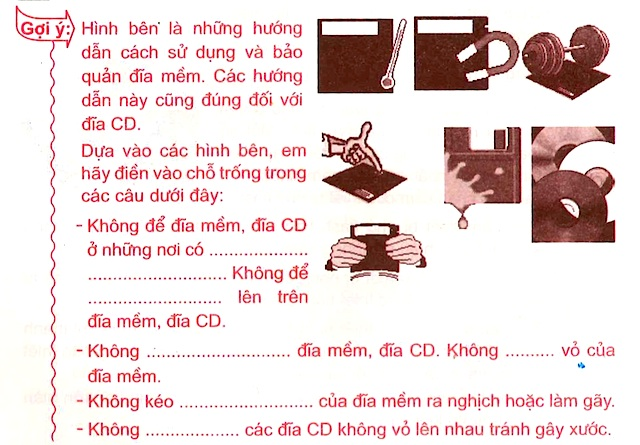
\includegraphics[width=\linewidth]{vietnam/vietnam_disketten.jpg}
\footnotesize{Unterrichtsmaterial über Disketten. Bildrechte: Volksrepublik Vietnam}
\end{center}
In der 3. Klasse lernen die Schüler Microsoft Windows zu benutzen. Vietnam ist zu 100 Prozent eine Windows XP Monokultur. Wahrscheinlich haben alle Windows-Lizenzen im Land die selbe Seriennummer. Verständlich, wenn man bedenkt dass eine Windows Lizenz soviel kostet wie ein Monatsgehalt.

Tippen (10-Finger-System) wird gelehrt mittels Microsoft Word. Ganz Vietnam verwendet englischsprachige Software in Schulen, was das Tippen lernen für die Kinder in diesem Alter erschwert.

Ab der 4. Klasse starten die Kinder mit der Programmiersprache \href{http://de.wikipedia.org/wiki/Logo_(Programmiersprache)}{\textbf{Logo}}. Zuerst mit Sequenzen von Befehlen, danach mit Schleifen (Loops). In der 5. Klasse schreiben die Kinder Prozeduren (Unterprogramme) welche Schleifen enthalten welche Unterprogramme aufrufen welche wiederum Schleifen enthalten.

Ein Vergleich mit den USA ist hier angebracht: Einige Besuche in San Francisco's 'magnet school for science and technology (Galileo Academy)' zeigten mir Schüler der 11. und 12. Klasse \footnote{entspricht 16-jährigen, Anm. d. Ü.} die sich schwer taten damit den \href{http://de.selfhtml.org/html/grafiken/einbinden.htm#referenz}{\textit{image tag (<img>)}} in Html zu verstehen. Computer Science Hausaufgaben waren von der Schuldirektion verboten worden.

Zu sagen dass ich beeindruckt war vom Computer Science Unterricht und Lehrplan in Vietnam's Grundschulen ist eine Untertreibung. Ich fragte was ich tun könne um zu helfen. Unerwarteterweise war die Antwort: "Software". Education-Software existiert in vietnamesischer Sprache überhaupt nicht, und es gibt auch kein Geld um sie zu kaufen, selbst wenn sie existieren würde.  Ich verbrachte den Rest meines Urlaubs damit, Software zu schreiben. Das Resultat ist \href{https://code.google.com/p/blockly/}{\textit{Blocky Maze [2]}}, welches in verschiedenen Sprachen läuft. Hier ein Link zur \href{http://blockly-demo.appspot.com/static/apps/maze/en.html?level=1}{Online-Demo-Version von \textit{Blocky Maze [3]}}. Blocky-Maze ist ein Selbst-Lern-Programm mit einer Reihe von Tutorials um Programmieren zu lernen. Verwendet werden Schleifen (loops) und Bedingungen (conditionals) sowie im Level 10 auch Listen, Variablen und Prozeduren. Ich musste alles auf eine CD brennen denn die Schule konnte sich keinen zuverlässigen Internetzugang leisten.

\begin{center}
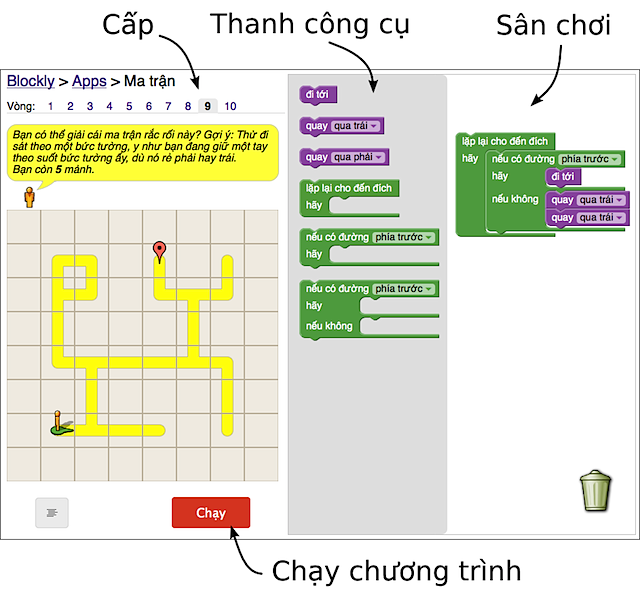
\includegraphics[width=\linewidth]{vietnam/vietnam_blocky.png}
\footnotesize{Blocky Maze, ein mehrsprachiges Programmierlernspiel. Bildrechte: Volksrepublik Vietnam}
\end{center}

Die Übergabe der Software zwei Wochen später war ein surreales Erlebnis: Im Büro des Schuldirektors zu sitzen ist als Erwachsener genauso furchterregend wie als Schulkind. Von der Wand sah der allgegenwärtige \href{http://goo.gl/fZATT3}{\textit{Ho Chi Minh}} auf mich herab. Vor der Schule begannen 1.500 Kinder ihre Morgengymnastik, zum Teil bestehend aus dem \href{http://www.youtube.com/watch?v=4xmV5uHWNag}{\textit{Chicken dance [4]}}.

Der Computer Science Lehrer war hoch erfreut und versprach mir Blocky schon am nächsten Tag im Unterricht einzusetzen. Wegen fehlendem Budget konnte sich die Schule keinen zweiten Computer Science Lehrer leisten, und nur die Hälfte der Kinder bekam Computer Science Unterricht. Ich fragte nach wieviel ein Computer Science Lehrer im Monat verdient: 100 Dollar. Daraufhin ging zum nächsten Bankomat und kaufte der Schule einen zweiten Computer Science Lehrer für ein Jahr.

Es stellte sich heraus dass man ziemlich populär wird wenn man Software und einen Lehrer spendet:
\begin{center}
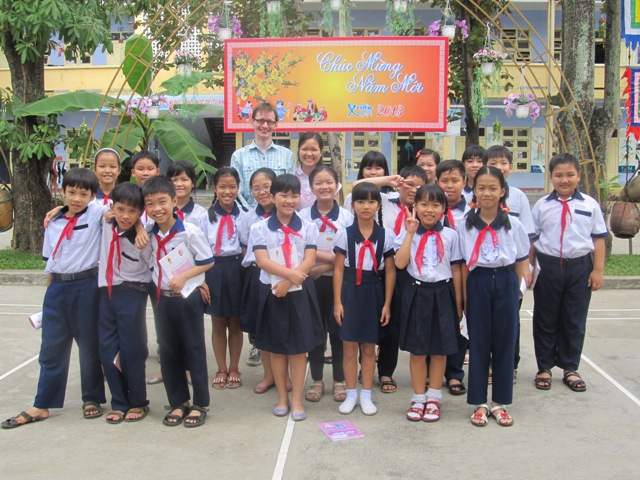
\includegraphics[width=\linewidth]{vietnam/vietnam_happy.jpg}
\footnotesize{happy Neil, happy students. Bildrechte: Volksrepublik Vietnam}
\end{center}

Wenn 5-grader in Vietnam mindestens genauso gut "performen" wie 11-grader in den USA, wie gut sind dann die 11-grader in Vietnam ? Ich ging in eine CS-Klasse in einer High School, auch diesmal ohne Vorankündigung. Die Klasse arbeitete an einem Test:

\begin{center}
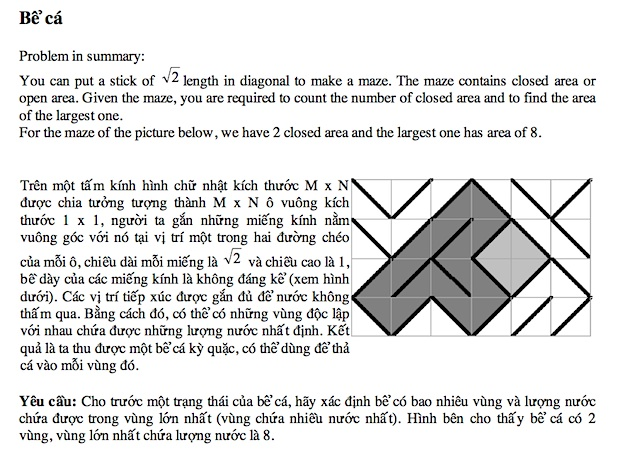
\includegraphics[width=\linewidth]{vietnam/vietnam_test.jpg}
\footnotesize{Computer Science Test. Bildrechte: Volksrepublik Vietnam}
\end{center}

Gegeben war eine Data File der ein Labyrinth mit diagonalen Wänden beschreibt. Aufgabe war es die Nummer der umschlossenen Flächen zu zählen und den Flächeninhalt der größten umschlossenen Fläche auszurechnen.

\subsection*{Data File:}
\large
\texttt{1000000010001000100000001 \\
0100000100010100010000010 \\
0010001000100010001000100 \\
0001010001000001000101000 \\
1000100010001000100010000 \\
0100000100010001010001000 \\
0010001000100010001000100 \\
0001010001000100000100010 \\
0000100010001000000010001 \\
0001000101000100000101000 \\
0010001000100010001000100 \\
0100010000010001010000010 \\
1000100010001000100010001 \\
0100000101000001000100010 \\
0010001000100010001000100 \\
0001010000010100010001000 \\
0000100000001000100010000 \\
}
\normalsize 


Nach meiner Rückkehr in die USA fragte ich einen senior engineer wie er die Prüfungsfrage einschätzen würde bezüglich eines Job-Interviews bei Google. Ohne dass er über die Herkunft der Frage Bescheid wusste antwortete mir der Senior Engineer die Frage entspräche dem oberen Drittel. Die Klasse in Vietnam hatte 45 Minuten Zeit eine Lösung in \href{http://de.wikipedia.org/wiki/Pascal_(Programmiersprache)}{\textbf{Pascal}} zu implementieren. Fast alle Schüler wurden fertig, und nur einige wenige brauchten zusätzliche fünf Minuten. Die Hälfte dieser Schüler würden den Google Job Interview Prozess überstehen.

Ich war in die High School in Vietnam hineingegangen mit der Bereitschaft zu helfen so gut ich konnte. Doch anstatt dass die Schule von mir und meiner Erfahrung profitierte, lernte ich etwas von den Schülern. Diese Schüler zeigten mir wie man Computer Science Unterricht machen sollte: \href{http://neil.fraser.name/news/2012/07/01/}{\textit{Fr\"uh mit Programmierunterricht beginnen [5]}}, verpflichtend für alle Schüler. Den Schülern die sich dafür interessieren unbegrenzt Raum zum wachsen geben.

Allerdings gibt es einen Haken im Vietnamesischen System. Die Einführung des Computerunterrichts in das Vietnamesische Schulsystem ist relativ neu. Es scheint so als ob es in allen Altersstufen gleichzeitig begann vor ein paar Jahren. Als ich eine Universität besuchte war ich nicht beeindruckt davon was die Studenten dort taten. Doch dies wird sich schnell ändern sobald die derzeitigen Schüler auf die Universitäten kommen mit ihrer bereits in der Schule erworbenen Programmiererfahrung.

\subsection*{Vergleich mit USA}
Der Zustand der Amerikanischen Computer Science Education ist erschreckend im Vergleich dazu.

Schulträger kämpfen darum \href{http://www.marylandpublicschools.org/MSDE/programs/esea/docs/TQ_Regulations/core_subjects.htm}{\textit{Computer Science [6]}} aus den Schulen herauszuhalten, denn jede Minute die mit CS verbracht wird fehlt bei den Kernfächern Englisch und Mathematik. Die Testergebnisse der Schüler in diesen Kernfächern beeinflussen das jährliche Schulbudget, deshalb wird Computerunterricht als Bedrohung wahrgenommen.

Lehrer weigern sich oft Computer Science vernünftig zu unterrichten, nicht zuletzt deshalb weil sie nichts davon verstehen.  \href{http://blog.carolynworks.com/?p=572}{\textit{Stattdessen unterrichten Sie Textverarbeitung und HTML und nennen dies dann Computer Science [7]}}.

Eltern opponieren gegen Computer Science Klassen weil deren Noten sich nicht direkt auf die akademischen Chancen ihrer Kinder auswirken. Dazu kommt  
\large 
\begin{quote}
\glqq 
Dass Eltern den Unterschied zwischen Kindern die Videospiele \href{http://www.youtube.com/watch?v=Lql-otlQfNo}{\textit{spielen [8]}} und Kindern die Videospiele \emph{programmieren} nicht erfassen.
\grqq
\end{quote}
\normalsize 
Schüler verlassen absichtlich die Computer Science Klassen da als \textbf{Nerd} zu gelten unglaublich unpopulär ist.

Das Resultat in den USA ist ein Widerstand gegen CS auf jeder Ebene. Diese Situation sinnvoll zu ändern erscheint unmöglich. Ich arbeite für die Bildungsabteilung von Google und die Geschichten mit denen unsere Externen Pädagogen zurückkommen sind schockierend und nicht veröffentlichbar. Wir \href{http://neil.fraser.name/news/2011/07/16/}{\textit{spenden Unsummen [9]}} und enorme Ressourcen mit minimalem Ergebnis.

Im Kontrast dazu ist es in Vietnam genau umgekehrt. Schulen, Lehrer, Eltern und Schüler sind lernwillig in einer Weise die ich in den USA nie erlebt habe. Es brauchte weniger als 10 Minuten um Blocky's Maze der Vietnamesischen CS Lehrerin zu zeigen . Ihre Kinder spielten es durch in einer Schulstunde, die meisten davon beendeten die ersten 9 Level. Und wollten mehr.

(Ende der Übersetzung)

In Neils Blog gibt es weitere, auf diesen Artikel bezugnehmende Postings, z.B. über \href{https://neil.fraser.name/news/2013/04/15/}{\textit{Neils Hochzeit [11]}} oder die \href{https://neil.fraser.name/news/2013/12/31/}{\textit{Popularität von Blockly [12]}}. 

\subsection*{Fachbegriffe:}

~~~\href{http://de.wikipedia.org/wiki/Diskette}{\textbf{Disketten}}: Magnetbeschichtete, scheibenförmige Datenträger, bis zum Aufkommen von USB-Sticks weit verbreitet. \\

\textbf{Logo}: wegweisende Programmiersprache, siehe auch RIS-Journal 001, Seite \pageref{austrianguy} \\

\textbf{Ho Chi Min}: Vietmanesischer Guerillaführer und Präsident, 1890-1969. \\

\textbf{Pascal}: beinahe ausgestorbene Programmiersprache, siehe auch RIS-Journal 001, Artikel \texttt{austrianguy} Seite \pageref{austrianguy} \\

\href{https://de.wikipedia.org/wiki/Nerd}{\textbf{Nerd}} engl. für Computerfreak, Fachidiot, Streber, Außenseiter.


\subsection*{Download, Feedback:}
\footnotesize{
Download: Ordner \texttt{vietnam} \Mundus\ \href{http://spielend-programmieren.at/risjournal/001}{spielend-programmieren.at/risjournal/001}\\
Startseite:\\
\href{http://spielend-programmieren.at/de:ris:001}{spielend-programmieren.at/de:ris:001}\\ 
\Letter\:  root@neil.fraser.name (Englisch)\\}
\normalsize
 

\subsection*{Lizenz, Quellen:}
\begin{wrapfigure}{l}{2.0cm}

\includegraphics[width=2cm]{vietnam/ccbysa88x31.png}
\end{wrapfigure}
Dieses Material steht unter der Creative-Commons-Lizenz Namensnennung - Weitergabe unter gleichen Bedingungen 4.0 International. Um eine Kopie dieser Lizenz zu sehen, besuchen Sie \url{http://creativecommons.org/licenses/by-sa/4.0/deed.de}. \\

\textbf{Quellen:} \\
{[}1{]}: \href{https://neil.fraser.name/news/2013/03/16/}{neil.fraser.name/news/2013/03/16/} \\
{[}2{]}: \href{https://code.google.com/p/blockly/}{code.google.com/p/blockly} \\
{[}3{]}: \href{https://blockly-demo.appspot.com/static/apps/index.html?lang=de}{http://goo.gl/gz5j50} \\
{[}4{]}: \href{http://www.youtube.com/watch?v=4xmV5uHWNag}{youtu.be/4xmV5uHWNag} \\
{[}5{]}: \href{http://neil.fraser.name/news/2012/07/01/}{neil.fraser.name/news/2012/07/01/} \\
{[}6{]}: \href{http://www.marylandpublicschools.org/MSDE/programs/esea/docs/TQ_Regulations/core_subjects.htm}{goo.gl/W1ixgX} \\
{[}7{]}: \href{http://blog.carolynworks.com/?p=572}{blog.carolynworks.com/?p=572} \\
{[}8{]}: \href{http://youtu.be/Lql-otlQfNo}{youtu.be/Lql-otlQfNo} \\
{[}9{]}: \href{https://neil.fraser.name/news/2011/07/16/}{neil.fraser.name/news/2011/07/16/} \\
{[}10{]}: \href{http://spielend-programmieren.at}{spielend-programmieren.at} \\
{[}11{]}: \href{https://neil.fraser.name/news/2013/04/15/}{neil.fraser.name/news/2013/04/15/} \\
{[}12{]}: \href{https://neil.fraser.name/news/2013/12/31/}{neil.fraser.name/news/2013/12/31/} \\
\end{multicols}
\SepRule
%-----------------------------------------------------------
\end{document}
